% !TeX spellcheck = en_GB
% \begin{figure}[t]
% 	\centering
%     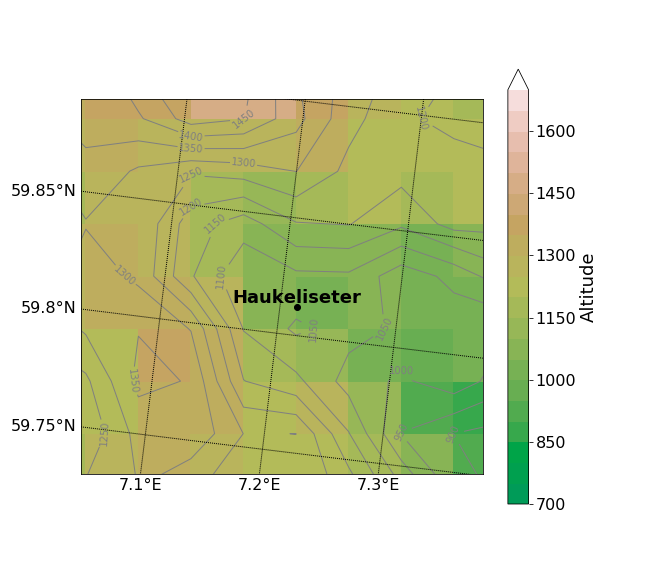
\includegraphics[trim={.3cm 2.2cm 1.8cm 2.4cm},clip,width=\textwidth]{./fig_Norway/MEPS_elevation_Haukeli}
%         \caption{}\label{fig:meps:site}
% \end{figure}

% \begin{wrapfigure}[14]{r}{0.55\textwidth}
% 	\vspace{-\normalbaselineskip}
% 	\centering
% 	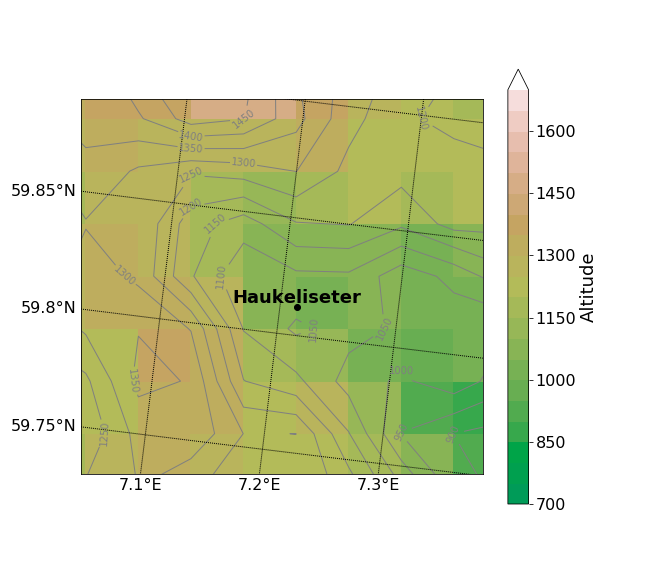
\includegraphics[trim={.3cm 2.2cm 1.8cm 2.4cm},clip,width=0.54\textwidth]{./fig_Norway/MEPS_elevation_Haukeli}
% 	%	\vspace{-10pt}
% 	\caption{Representation of the topography around measurement site Haukeliseter in MEPS. Contours and shading present the elevation of the grid cells.}\label{fig:meps:site}
% 	\vspace{-\normalbaselineskip}
% \end{wrapfigure}

% !TeX spellcheck = en_GB
\begin{figure}[ht!]
	\centering
    \begin{subfigure}[b]{0.53\textwidth}
    	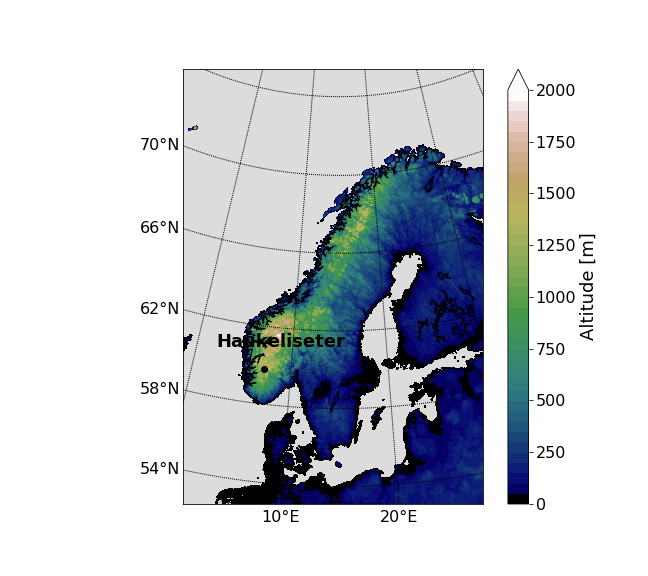
\includegraphics[trim={4.cm 1.8cm 0cm 2.cm},clip,width=1.05\textwidth]{./fig_Norway/Norway_elevation_MEPS}
        \caption{}\label{fig:meps:Norway}
    \end{subfigure}
    \begin{subfigure}[b]{0.46\textwidth}
        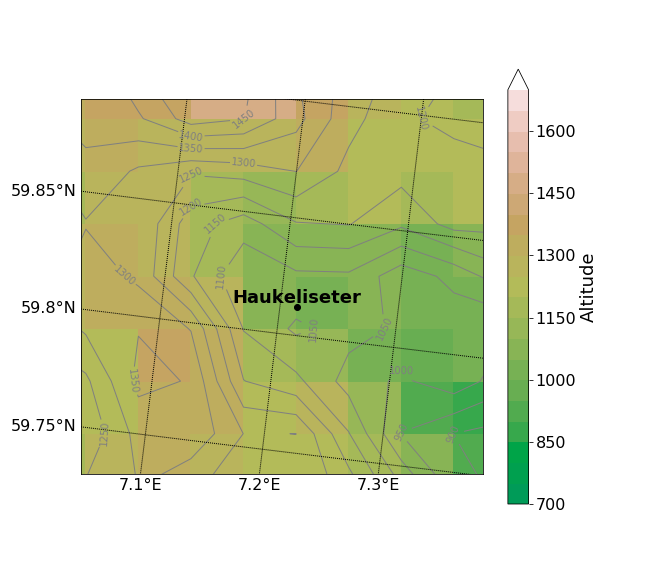
\includegraphics[trim={.3cm 2.2cm 1.8cm 2.4cm},clip,width=\textwidth]{./fig_Norway/MEPS_elevation_Haukeli}
        \caption{}\label{fig:meps:site}
      \end{subfigure}
	\caption{\protect\subref{fig:meps:Norway}: Elevation map of MEPS model domain. \protect\subref{fig:meps:site}: Representation of the topography around the measurement site Haukeliseter in MEPS. Contours and shading present the elevation of the grid cells.}\label{fig:meps_site}
\end{figure} 